\section{Parallel Knuth Shuffle with Early Termination}

\subsection{Changes from Shun et al.}

\begin{frame}{Can we do better?}
  \begin{itemize}
    \item Using Shun et al.'s parallel Knuth Shuffle: \(\O(n)\) work and \(\O(\log n)\) span.
    \item Still proportional to \(n\)
  \end{itemize}
  \vspace{2em}
  \begin{center}
    \textbf{New idea:} Stop after \(k\) elements swapped
  \end{center}
\end{frame}

\begin{frame}{Parallel Knuth Shuffle with Early Termination}
  \begin{algorithm}[H]
    \caption{\textsc{ParPermute}}
    \begin{algorithmic}
      \Input{Array \(A\), Swap targets \(H\)}

      \State{\(I \gets [1, 2, \ldots, k]\)} \Comment{\(k\) instead of \(n\)}
      \State{\(R \gets [n, n, \ldots, n]\) of length \(n\)}
      \While{\(I\) is not empty}
        \ParFor{\(i \in I\)}
          \State{\textsc{Reserve(\(R, i\))}}
        \EndParFor
        \ParFor{\(i \in I\)}
          \State{\textsc{Commit(\(R, i\))}}
        \EndParFor
        \State{Remove committed indices from \(I\)}
      \EndWhile
    \end{algorithmic}
  \end{algorithm}
\end{frame}

\subsection{Span Analysis}

\begin{frame}{Length of Dependency Chain}
  \begin{definition}[Length of Dependency Chain]
    Let \(\mathcal{L}(t)\) be the length of the dependency chain starting at
    index \(t\). 
    \[
      \mathcal{L}(t) = \begin{cases}
        0 & \text{if \(t \geq k\)} \\
        1 + \mathcal{L}(H[t]) & \text{otherwise}
      \end{cases}
    \]
  \end{definition}
  \vspace{1em}
  E.g., when \(k=4\), \(\mathcal{L}(1) = 2\) with 1, 3, and 8 in the chain and \(\mathcal{L}(4) = 0\).
  \begin{figure}
    \begin{center}
      \begin{tikzpicture}[
        arr-elm/.style = {draw, rectangle, text centered, minimum size=0.5em}, 
        node distance = 1.25em
      ]
        \node[arr-elm,fill=Processing] (1) {3};
        \node[arr-elm,right of=1] (2) {5};
        \node[arr-elm,right of=2,fill=Processing] (3) {8};
        \node[arr-elm,right of=3,fill=red!15!white] (4) {6};
        \node[arr-elm,right of=4] (5) {7};
        \node[arr-elm,right of=5] (6) {7};
        \node[arr-elm,right of=6] (7) {7};
        \node[arr-elm,right of=7] (8) {8};

        \draw[->] (1.north) .. controls +(up:5mm) and +(up:5mm) .. (3.north);
        \draw[->] (3.north) .. controls +(up:5mm) and +(up:5mm) .. (8.north);

        \draw[->] (4.south) .. controls +(down:5mm) and +(down:5mm) .. (6.south);
      \end{tikzpicture}
    \end{center}
    % \caption{\(H = [
    %   \underset{1}{3}, 
    %   \underset{2}{5}, 
    %   \underset{3}{8}, 
    %   \underset{4}{6}, 
    %   \underset{5}{7}, 
    %   \underset{6}{7}, 
    %   \underset{7}{7}, 
    %   \underset{8}{8} 
    % ]\)}
  \end{figure}
\end{frame}

\begin{frame}{Length of Dependency Chain}
  \begin{lemma}[Expected Length of Dependency Chain]
    Let \(\Lb(t)\) be the expected length of the dependency chain starting
    at index \(t\).
    \[ \Lb(t-1) = \Lb(t) + \frac{1}{n+2-t} \]
  \end{lemma}
\end{frame}

\begin{frame}{Length of Dependency Chain}
  \begin{proofs}
    By definition,
    \begin{align*}
      \Lb(t) &= \frac{1}{n-(t-1)} \left(\sum_{i=t}^k \Lb(i)\right) + 1 \\ 
      % \Lb(t) &= \frac{1}{n+1-t} \left(\Lb(t) + \Lb(t+1) + \cdots + \Lb(k)\right) + 1 \\
      % (n+1-t)\Lb(t) &= \Lb(t) + \Lb(t+1) + \cdots + \Lb(k) + n+1-t
      % \numberthis\label{eqn:ex-len-t}
    \end{align*}

    E.g., \(H[1]\) picks from \(\{1, 2, \ldots, 8\}\) w.p.
    \(\frac{1}{8-(1-1)} = \frac{1}{8}\) each

    \begin{figure}
      \begin{center}
        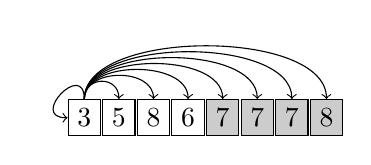
\begin{tikzpicture}[
          arr-elm/.style = {draw, rectangle, text centered, minimum size=0.5em}, 
          node distance = 1.25em
        ]
          \node[arr-elm] (1) {3};
          \node[arr-elm,right of=1] (2) {5};
          \node[arr-elm,right of=2] (3) {8};
          \node[arr-elm,right of=3] (4) {6};
          \node[arr-elm,right of=4,fill=black!20!white] (5) {7};
          \node[arr-elm,right of=5,fill=black!20!white] (6) {7};
          \node[arr-elm,right of=6,fill=black!20!white] (7) {7};
          \node[arr-elm,right of=7,fill=black!20!white] (8) {8};

          \draw[->] (1.north) .. controls +(up:5mm) and +(left:5mm) .. (1.west);
          \draw[->] (1.north) .. controls +(up:3mm) and +(up:3mm) .. (2.north);
          \draw[->] (1.north) .. controls +(up:4mm) and +(up:4mm) .. (3.north);
          \draw[->] (1.north) .. controls +(up:5mm) and +(up:5mm) .. (4.north);
          \draw[->] (1.north) .. controls +(up:6mm) and +(up:6mm) .. (5.north);
          \draw[->] (1.north) .. controls +(up:7mm) and +(up:7mm) .. (6.north);
          \draw[->] (1.north) .. controls +(up:8mm) and +(up:8mm) .. (7.north);
          \draw[->] (1.north) .. controls +(up:9mm) and +(up:9mm) .. (8.north);
        \end{tikzpicture}
      \end{center}
    \end{figure}
  \end{proofs}
\end{frame}

\begin{frame}{Length of Dependency Chain}
  \begin{proofs}
    By definition,
    \begin{align*}
      \Lb(t) &= \frac{1}{n-(t-1)} \left(\sum_{i=t}^k \Lb(i)\right) + 1 \\ 
      \Lb(t) &= \frac{1}{n+1-t} \left(\Lb(t) + \Lb(t+1) + \cdots + \Lb(k)\right) + 1 \\
      (n+1-t)\Lb(t) &= \Lb(t) + \Lb(t+1) + \cdots + \Lb(k) + (n+1-t)
      \numberthis\label{eqn:ex-len-t}
    \end{align*}
  \end{proofs}
\end{frame}

\begin{frame}{Length of Dependency Chain}
  \begin{proofs}
    Similarly,
    \begin{align*}
      \Lb(t-1) &= \frac{1}{n+2-t} \left(\sum_{i=t-1}^k \Lb(i)\right) + 1 \\ 
      \Lb(t-1) &= \frac{1}{n+2-t} \left(\Lb(t-1) + \Lb(t) + \Lb(t+1) + \cdots + \Lb(k)\right) + 1 \\ 
      (n+2-t)\Lb(t-1) &= \Lb(t-1) + \Lb(t+1) + \cdots + \Lb(k) + n+2-t
      \numberthis\label{eqn:ex-len-tmn}
    \end{align*}
  \end{proofs}
\end{frame}

\begin{frame}{Length of Dependency Chain}
  \begin{proof}
    Subtracting (\ref{eqn:ex-len-t}) from (\ref{eqn:ex-len-tmn}) yields
    \begin{align*}
      \Lb(t-1) &= \Lb(t) + \frac{1}{n+2-t}
    \end{align*}
  \end{proof}
\end{frame}

\begin{frame}{Expected Longest Chain}
  \begin{theorem}[Longest Chain of Dependency]
    The longest chain of dependency, i.e. \(\Lb(1)\), has length
    \(\O\left(\log\left(\frac{n}{n-k}\right)\right)\).
  \end{theorem}
\end{frame}

\begin{frame}{Expected Longest Chain}
  \begin{proof}
    \[
      \begin{aligned}
        \Lb(1) &= \Lb(2) + \frac{1}{n} \\ 
               &= \Lb(3) + \frac{1}{n-1} + \frac{1}{n} \\ 
               &\ \ \vdots \\ 
               &= \cancelto{0}{\Lb(k)} + \frac{1}{n+1-k} + \cdots + \frac{1}{n} \\
               &= H_n - H_{n+1-k} \\
               &\leq \ln n - \ln (n+1-k) = \O\left(\log\left(\frac{n}{n-k}\right)\right)
      \end{aligned}
    \]
  \end{proof}
\end{frame}

\begin{frame}{Parallel Knuth Shuffle with Early Termination}
  Implications:
  \begin{itemize}
    \item With early termination, span is \(\O\left(\log\left(\frac{n}{n-k}\right)\right)\)
    \item If \(k \ll n\), span approaches \(\O(1)\)
    \item If \(k \approx n\), span approaches \(\O(\log n)\)
  \end{itemize}
\end{frame}
